We developed a REST API that provides encryption and decryption services using attribute-based encryption. The API allows clients to encrypt data with an access policy and decrypt the data if they satisfy the policy. The API is implemented using Flask, a lightweight web framework for Python, and uses the Charm-Crypto library for pairing-based cryptography. The API endpoints are secured using HashiCorp Vault to manage cryptographic keys securely.

\section{Libraries and Tools Used}

The following libraries and tools were used in the implementation:

\begin{itemize}
    \item \textbf{Charm-Crypto}: A Python library for pairing-based cryptography, used to implement the attribute-based encryption scheme.
    \item \textbf{Flask}: A lightweight web framework for building the API endpoints for encryption and decryption.
    \item \textbf{Flask-RESTX}: An extension for Flask that adds support for creating REST APIs.
    \item \textbf{PyCryptodome}: A self-contained Python package of low-level cryptographic primitives, used for AES encryption and decryption.
    \item \textbf{HashiCorp Vault}: A tool for securely storing and accessing secrets, used to manage cryptographic keys.
\end{itemize}


\section{Setup authority}
This method is used to set up an authority in the system. The authority is identified by a unique uppercase alphanumeric string. The authority's public and private keys are generated by Charm-Crypto MaabeRW15\cite{rouselakis2015efficient} scheme and stored in HashiCorp Vault. The authority private key is used for key generation for each attribute. The public key is used for encryption by the clients.

For simplicity in developing and testing, the authority's private key is stored in HashiCorp Vault. In a production scenario the private key should be stored securely by the authority and provided to the system only when needed.

\begin{algorithm}
    \caption{Setup Authority}
    \label{alg:setup_authority}
    \begin{algorithmic}[1]
    \Procedure{SetupAuthority}{authority}
        \State $pk, sk \gets \textsc{generateAuthorityKeys}()$
        \State $\textsc{storeAuthorityKeys}(authority, pk, sk)$
    \EndProcedure
    \end{algorithmic}
\end{algorithm}

\section{Keygen}
This method is used to generate a key for an attribute and associate it with an user. The key is generated using the authority's private key and the attribute name. The key is stored in HashiCorp Vault and can be used for decryption.

\begin{algorithm}
    \caption{Keygen}
    \label{alg:keygen}
    \begin{algorithmic}[1]
    \Procedure{Keygen}{authority, attribute, user}
        \State $sk \gets \textsc{retrieveAuthorityPrivateKey}(authority)$
        \State $K \gets \textsc{generateKey}(sk, attribute)$
        \State $\textsc{storeKey}(user, K)$
    \EndProcedure
    \end{algorithmic}
\end{algorithm}


\section{Encrypt}
This method is used to encrypt a payload with an access policy. The access policy is specified as a string containing a boolen expression of attributes and logical operators which should be sattisfied to decrypt the payload. The method retrieves the public keys of the authorities associated with the attributes in the policy and generates a symmetric key as a random member of $G_T$. This element is then used to generate an AES symmetric key to encrypt the payload. The original $G_T$ element is then encrypted by MaabeRW15 scheme using the public keys of the authorities and the access policy. The encrypted element and the AES encrypted payload are returned to the client. This guarantees that the symmetric key used to encrypt the payload is only accessible to users with the required attributes.

\begin{figure}
\label{fig:encrypt_process}
\centering
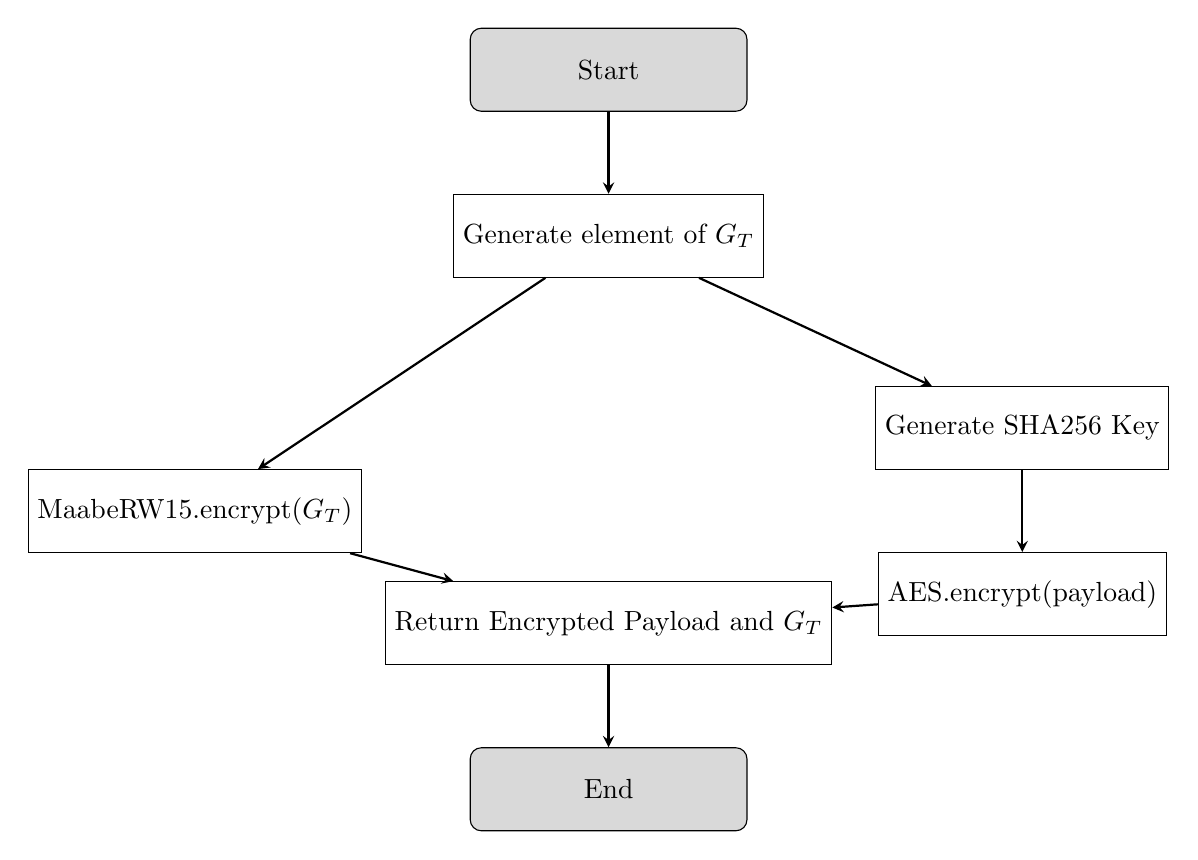
\begin{tikzpicture}[node distance=7em]
    \usetikzlibrary{positioning, fit}

    % Define styles
    \tikzset{
        startstop/.style = {rectangle, rounded corners, minimum width=10em, minimum height=3em, text centered, draw=black, fill=gray!30},
        process/.style = {rectangle, minimum width=10em, minimum height=3em, text centered, draw=black, fill=white!30},
        decision/.style = {diamond, minimum width=10em, minimum height=3em, text centered, draw=black, fill=green!30},
        arrow/.style = {thick,->,>=stealth}
    }
    
    % Nodes
    \node (start) [startstop] {Start};
    \node (gt) [process, below of=start, node distance=6em] {Generate element of $G_T$};
    \node (sha) [process, below right of=gt, xshift=10em, yshift=-2em] {Generate SHA256 Key};
    \node (aes) [process, below of=sha, node distance=6em] {AES.encrypt(payload)};
    \node (maabe) [process, below left of=gt, xshift=-10em, yshift=-5em] {MaabeRW15.encrypt($G_T$)};
    \node (return) [process, below of=gt, node distance=14em] {Return Encrypted Payload and $G_T$};
    \node (stop) [startstop, below of=return, node distance=6em] {End};
    
    % Arrows
    \draw [arrow] (start) -- (gt);
    \draw [arrow] (gt) -- (sha);
    \draw [arrow] (gt) -- (maabe);
    \draw [arrow] (sha) -- (aes);
    \draw [arrow] (maabe) -- (return);
    \draw [arrow] (aes) -- (return);
    \draw [arrow] (return) -- (stop);
\end{tikzpicture}
\caption{Encrypt Process}
\end{figure}

\subsection{Process of Creating the AES Key}

The process of creating the AES key involves the generation of a symmetric key using the attribute-based encryption scheme and hashing the key to the appropriate length for AES encryption.

\begin{enumerate}
    \item \textbf{Generate Symmetric Key}: A symmetric key is generated using the attribute-based encryption scheme. This key is derived based on the specified access policy and the public keys of the authorities.
    \item \textbf{Serialize Symmetric Key}: The symmetric key is serialized to a hexadecimal string for further processing.
    \item \textbf{Hash Symmetric Key}: The serialized symmetric key is hashed using the SHA-256 hash function to produce a 256-bit key suitable for AES encryption.
\end{enumerate}

Mathematically, the process can be described as follows:

\begin{equation}
\text{hashed\_key} = \text{SHA-256}(\text{serialized\_symmetric\_key})
\end{equation}
\subsection{AES Encryption and Decryption}

The AES encryption and decryption process involves using the hashed symmetric key to encrypt and decrypt the payload data. The steps are as follows:

\subsubsection{Encryption}

\begin{enumerate}
    \item \textbf{Initialize Pairing Group}: Initialize the pairing group \(G_T\).
    \item \textbf{Generate Random Element}: Generate a random element \(gt\) in \(G_T\).
    \item \textbf{Retrieve Public Keys}: Retrieve the public keys from the key manager for the specified authorities.
    \item \textbf{Encrypt with MA-ABE}: Use the MA-ABE scheme to encrypt the random element \(gt\) with the public keys and access policy.
    \item \textbf{Serialize Symmetric Key}: Serialize the symmetric key to a hexadecimal string.
    \item \textbf{Hash Symmetric Key}: Hash the serialized symmetric key using SHA-256 to produce a 256-bit key.
    \item \textbf{Initialize AES Cipher}: Initialize an AES cipher object in CBC mode using the hashed symmetric key.
    \item \textbf{Pad Payload}: Pad the payload data to ensure it is a multiple of the AES block size.
    \item \textbf{Encrypt Payload}: Encrypt the padded payload using the AES cipher.
\end{enumerate}

\begin{algorithm}
    \caption{Encryption Process}
    \label{alg:encryption_process}
    \scriptsize
    \begin{algorithmic}[1]
    \Procedure{Encrypt}{payload, policy}
        \State $K_{G_T} \gets \textsc{Random}(G_T)$
        \State $A \gets \textsc{getAuthorities}(\text{policy})$
        \Comment{Attributes in the policy are defined as "<attribute>@<authority>"}
        \State $K_{\textsc{A}} \gets \textsc{retrievePublicKeys}(\text{authorities})$
        \State $K_{\textsc{SHA}} \gets \textsc{SHA256}(K_{G_T})$
        \State $E_{K_{G_T}} \gets \textsc{maabe.Encrypt}(\text{publicKeys}, K_{G_T}, \text{policy})$
        \State $E_{\text{payload}} \gets \textsc{AES.encrypt}(\text{payload}, K_{G_T})$
        \State \Return $E_{K_{G_T}}, E_{\text{payload}}$
    \EndProcedure
    \end{algorithmic}
\end{algorithm}


\subsubsection{Decryption}

\begin{enumerate}
    \item \textbf{Initialize AES Cipher}: An AES cipher object is initialized in CBC mode using the hashed symmetric key.
    \item \textbf{Decrypt Ciphertext}: The ciphertext is decrypted using the AES cipher.
    \item \textbf{Unpad Decrypted Data}: The decrypted data is unpadded to retrieve the original payload.
\end{enumerate}

\begin{algorithm}
    \caption{Decryption Process}
    \label{alg:decryption_process}
    \scriptsize
    \begin{algorithmic}[1]
    \Procedure{Decrypt}{$E_{K_{G_T}}$, $E_{\text{payload}}$, $K_{\text{user}}$}
        \State $K_{G_T} \gets \textsc{maabe.Decrypt}(E_{K_{G_T}}, K_{\text{user}})$
        \State $K_{\textsc{SHA}} \gets \textsc{SHA256}(K_{G_T})$
        \State $payload \gets \textsc{AES.decrypt}(E_{\text{payload}}, K_{G_T})$
        \State \Return $payload$
    \EndProcedure
    \end{algorithmic}
\end{algorithm}
